\documentclass[a4paper,12pt]{article}
\usepackage[utf8]{inputenc}
\usepackage[spanish]{babel}
\usepackage{graphicx}
\usepackage{amsmath}
\usepackage{mathptmx} % Paquete para cambiar a Times New Roman
\usepackage[left=2.54cm, right=2.54cm, top=2.54cm, bottom=2.54cm]{geometry}
\usepackage{tocbibind} % Para que el índice aparezca en el ToC
\usepackage{float} % Para obligar la posición de las figuras
\usepackage{listings} % Para el código fuente
\usepackage{setspace} % Paquete para configurar el interlineado
\usepackage{sectsty} % Paquete para configurar el tamaño de los títulos

\lstset{
  basicstyle=\ttfamily\footnotesize,
  breaklines=true,
  frame=single,
  language=Python,
  captionpos=b
}

\doublespacing % Establece el interlineado a doble espacio

% Configuración de los títulos
\allsectionsfont{\normalsize}

\begin{document}

% Portada con formato APA
\begin{titlepage}
    \begin{center}
        \textbf{\large “Año del Bicentenario, de la consolidación de nuestra Independencia, y de la conmemoración de las heroicas batallas de Junín y Ayacucho”}\\
        \vspace{0.5cm}
        \textbf{\large Universidad Nacional Mayor de San Marcos}\\
        \vspace{0.5cm}
        \textbf{\large Universidad del Perú, Decana de América}\\
        \vspace{0.5cm}
        
\includegraphics[height=4cm]{unmsm.png}\\ % Ajusta el tamaño de la imagen
        \vspace{5mm}
        \textbf{\large Facultad de Ingeniería de Sistemas e Informática}\\
        \vspace{0.5cm}
        \textbf{\large Escuela Profesional de Ingeniería de Sistemas}\\
        \vspace{0.5cm}
        \textbf{\large Proyecto de fin de curso}\\
        \vspace{0.5cm}
        \textbf{\large Profesor: Luis Guerra Grados}\\
        \vspace{1cm}
    \end{center}

    \begin{center}
        \textbf{\large Integrantes del grupo N° 2:}\\
        \vspace{0.5cm}
        {\large Campos García, Henry Leonardo}\\
        \vspace{0.3cm}
        {\large Escribas Alan, Daniel Leonardo}\\
        \vspace{0.3cm}
        {\large Meléndez Blas, Jhair Roussell}\\
        \vspace{0.3cm}
        {\large Morales Damasco, Cristian Ricardo}\\
        \vspace{0.3cm}
        {\large Ortis Herrera, Fabrizio Peter}\\
        \vspace{1cm}
        {\large 23 / junio / 2024}
    \end{center}
\end{titlepage}


\newpage
\tableofcontents
\newpage

\section{Introducción}
Imagina estar en una tienda y necesitar dar el cambio exacto con la menor cantidad de monedas posible; en una empresa de transporte marítimo que debe seleccionar las mercancías más valiosas sin sobrecargar el barco; o en un repartidor que necesita encontrar la ruta más corta para entregar pedidos a varias casas. Estos escenarios cotidianos ilustran problemas de optimización complejos que pueden ser resueltos eficientemente mediante la programación dinámica. Esta técnica se basa en dividir problemas grandes en subproblemas más pequeños y manejables reutilizando las soluciones de estos subproblemas para construir una solución óptima de manera eficiente.

La programación dinámica no solo es eficaz sino también versátil se puede encontrar aplicaciones en diversas áreas como la logística la gestión de recursos la ingeniería de redes y la toma de decisiones. La complejidad algorítmica de los algoritmos de programación dinámica varía según la estructura del problema y el tamaño de los parámetros de entrada. Esto significa que la eficiencia de estos algoritmos está directamente relacionada con el tamaño del problema haciendo que la programación dinámica sea una herramienta invaluable en la resolución de problemas de gran escala.

En ese sentido el presente informe se centra en tres problemas clásicos resueltos mediante programación dinámica: el problema del cambio de monedas, el problema de la mochila y el problema de las distancias más cortas. A través del análisis y la implementación de algoritmos para estos problemas se demuestra la eficacia de la programación dinámica en la optimización de recursos y la toma de decisiones ofreciendo soluciones prácticas y eficientes en contextos diversos.

\section{Objetivos}
\subsection{Objetivo General}
Desarrollar y analizar algoritmos eficientes basados en programación dinámica para resolver problemas clásicos de optimización demostrando su aplicabilidad y eficiencia en diferentes contextos.

\subsection{Objetivos Específicos}
\begin{itemize}
    \item Implementar un algoritmo de programación dinámica para resolver el problema del cambio de monedas con restricciones en la cantidad disponible.
    \item Desarrollar un algoritmo basado en programación dinámica para maximizar los ingresos en el problema de la mochila.
    \item Aplicar el algoritmo de Floyd-Warshall para encontrar las rutas de menor coste en un grafo optimizando la logística de entrega.
    \item Analizar la complejidad algorítmica de cada algoritmo implementado destacando los factores que afectan su rendimiento.
\end{itemize}

\section{Planteamiento del Problema}
¿De qué manera la programación dinámica resulta ser una solución eficiente y precisa para resolver problemas de optimización como el cambio de la moneda, el problema de la mochila o la selección de rutas óptimas en diversos contextos comerciales?

\section{El problema del cambio de monedas}
El problema del cambio de monedas, un desafío clásico en el campo de la optimización combinatoria y las ciencias de la computación, involucra determinar el número mínimo de monedas que se requieren para sumar una cantidad específica de dinero. Este problema se complica aún más cuando las monedas disponibles están limitadas en cantidad. La programación dinámica ofrece una metodología robusta para abordar este tipo de problemas permitiendo una solución eficiente y efectiva.

\subsection{Ejemplo 1}
Un cliente paga una cuenta de 6.20 soles con un billete de 10 soles. El cajero necesita dar el cambio con la menor cantidad de monedas posible. Las denominaciones disponibles son monedas de 1 sol, 50 céntimos, 20 céntimos y 10 céntimos con cantidades limitadas de cada una. El reto es calcular la forma óptima de entregar 3.80 soles de vuelto usando las denominaciones mencionadas. Considere que tiene 2 monedas de 1 sol, seis de 50 céntimos, cinco de 20 céntimos, y diez de 10 céntimos.

\subsubsection{Código}
\begin{lstlisting}
def min_coins_change(total, denominations, counts):
    # Convertimos las cantidades a centimos para manejarlas como enteros
    total_cents = int(total * 100)
    denominations_cents = [int(d * 100) for d in denominations]

    # Inicializamos la tabla de DP con infinito para todas las cantidades
    # excepto para 0 que necesita 0 monedas
    dp = [float('inf')] * (total_cents + 1)
    dp[0] = 0

    # Para rastrear el uso de las monedas correctamente
    used_coins = [[0 for _ in denominations] for _ in range(total_cents + 1)]

    # Procesamos cada tipo de moneda
    for i, coin in enumerate(denominations_cents):
        for j in range(coin, total_cents + 1):
            if dp[j - coin] != float('inf') and counts[i] > used_coins[j - coin][i]:
                if dp[j] > dp[j - coin] + 1:
                    dp[j] = dp[j - coin] + 1
                    used_coins[j] = used_coins[j - coin][:]
                    used_coins[j][i] += 1


    if dp[total_cents] == float('inf'):
        return "No se puede dar el cambio exacto"
    else:
        return dp[total_cents], used_coins[total_cents]

# Denominaciones de las monedas disponibles y sus cantidades
denominations = [1.0, 0.50, 0.20, 0.10]  # en soles
counts = [2, 6, 5, 10]  # cantidad de monedas disponibles

# Cantidad total a devolver
total_change = 3.80  # en soles


min_coins, coin_usage = min_coins_change(total_change, denominations, counts)

print("Numero minimo de monedas:", min_coins)
print("Uso de monedas:", coin_usage)
\end{lstlisting}

\subsubsection{Resultado}
\begin{figure}[H]
    \centering
    
\includegraphics[width=0.8\textwidth]{resultado_imagen.png}
    \caption{resultado del codigo Python.}
    \label{fig:resultado}
\end{figure}

\subsubsection{Análisis de complejidad}
\begin{figure}[H]
    \centering
    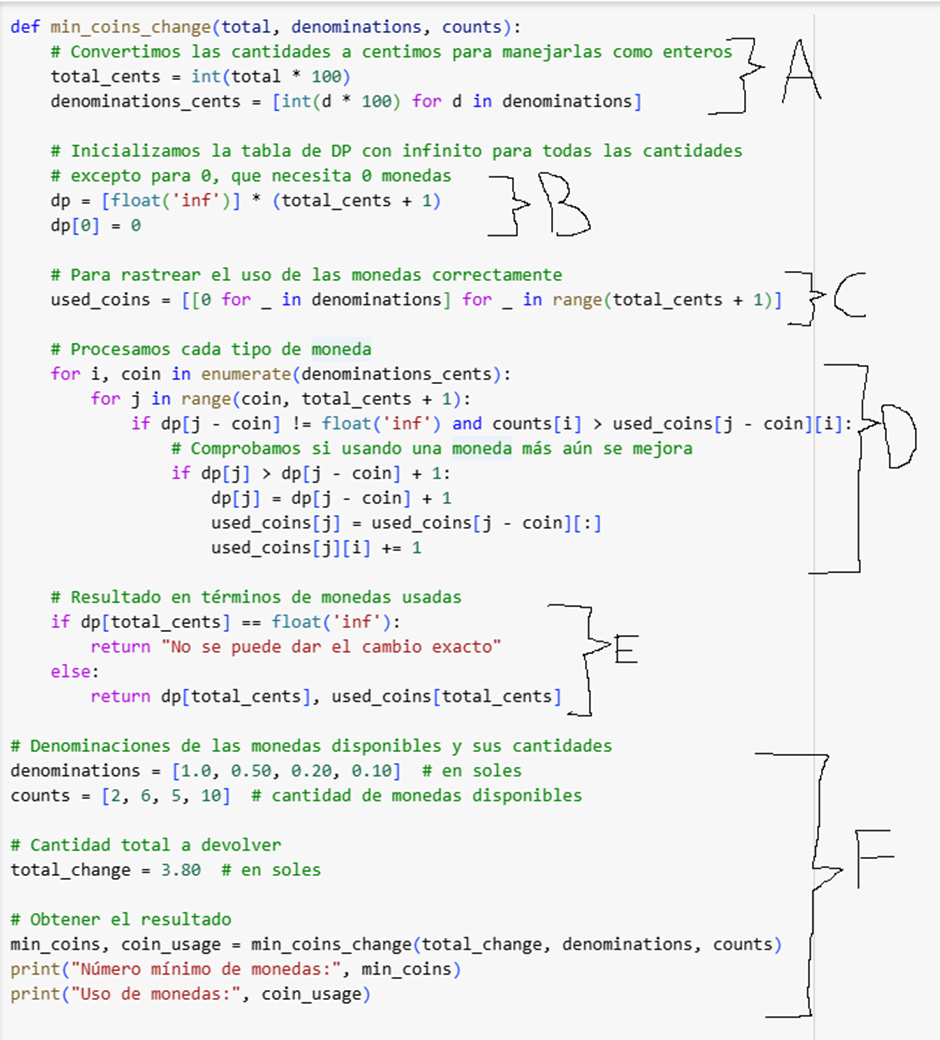
\includegraphics[width=0.8\textwidth]{complejidad_1.png}
    \caption{Analisis del codigo.}
    \label{fig:complejidad1}
\end{figure}

\begin{figure}[H]
    \centering
    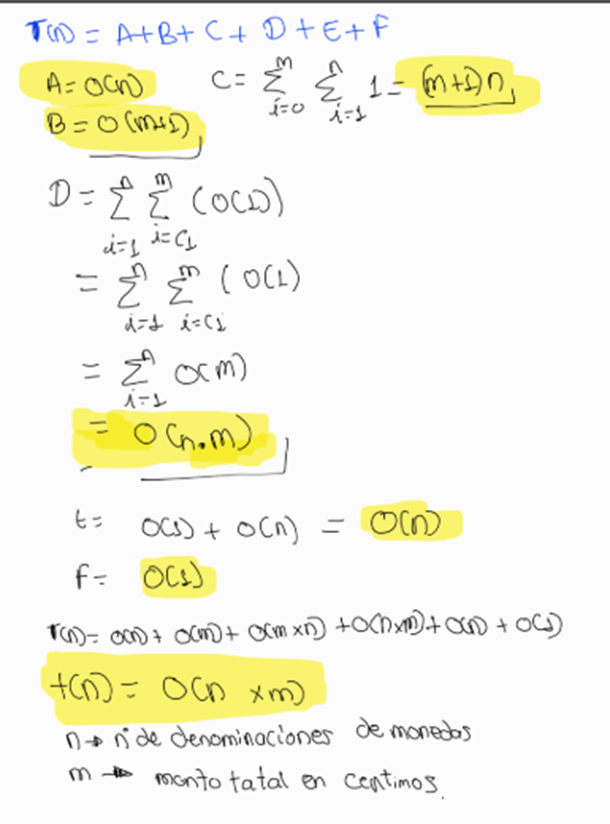
\includegraphics[width=0.8\textwidth]{complejidad_2.png}
    \caption{analisis del codigo.}
    \label{fig:complejidad2}
\end{figure}

La complejidad de este algoritmo está dada por la cantidad de denominaciones y la cantidad total a devolver, lo que resulta en una complejidad de \(O(n \cdot m)\), donde \(n\) es el número de denominaciones y \(m\) es la cantidad total a devolver.

\subsection{Ejemplo 2}
En primer lugar, debemos pensar cómo plantear el problema de forma incremental. Consideramos el tipo de moneda de mayor valor, \(X_N\). Si \(X_N > C\) entonces la descartamos y pasamos a considerar monedas de menor valor. Si \(X_N \leq C\) tenemos dos opciones: o tomar una moneda de tipo \(X_N\) y completar la cantidad restante \(C - X_N\) con otras monedas, o no tomar ninguna moneda de tipo \(X_N\) y completar la cantidad \(C\) con monedas de menor valor. De las dos opciones, nos quedamos con la que requiera un número menor de monedas. El problema lo podemos expresar de la siguiente forma cuando consideramos \(N\) tipos de monedas:

\[
Cambio(N, C) = 
\begin{cases} 
cambio(N-1, C) & \text{si } X_N > C \\
\min\{cambio(N-1, C), cambio(N, C - X_N) + 1\} & \text{si } X_N \leq C 
\end{cases}
\]

Podemos razonar análogamente para monedas de valores \(k\) menores que \(N\) y para cantidades \(C'\) menores que \(C\):

\[
Cambio(k, C') = 
\begin{cases} 
cambio(k-1, C') & \text{si } X_k > C' \\
\min\{cambio(k-1, C'), cambio(N, C' - X_k) + 1\} & \text{si } X_k \leq C' 
\end{cases}
\]

Llegamos a los casos base de la recurrencia cuando completamos la cantidad \(C\):

\[
cambio(k, 0) = 0 \quad \text{si } 0 \leq k \leq n
\]

o cuando ya no quedan más tipos de monedas por considerar, pero aún no se ha completado la cantidad \(C\):

\[
cambio(0, C') = \infty \quad \text{si } 0 < C' \leq C
\]

Podemos construir una tabla para almacenar los resultados parciales que tenga una fila para cada tipo de moneda y una columna para cada cantidad posible entre 1 y \(C\). Cada posición \(t[i,j]\) será el número mínimo de monedas necesario para dar una cantidad \(j\) con \(0 \leq j \leq C\) utilizando solo monedas de los tipos entre 1 e \(i\), con \(0 \leq i \leq n\). La solución al problema será, por tanto, el contenido de la casilla \(t[N, C]\). Para construir la tabla, empezamos rellenando los casos base \(t[i, 0] = 0\), para todo \(i\) con \(0 \leq i \leq n\). A continuación, podemos rellenar la tabla bien por filas de izquierda a derecha, o bien por columnas de arriba a abajo.

Siguiendo el método de la \textbf{programación dinámica}, se rellenará una tabla con las filas correspondientes a cada valor para las monedas y las columnas con valores desde el 1 hasta el \(N\) (12 en este caso). Cada posición \((i, j)\) de la tabla nos indica el número mínimo de monedas requeridas para devolver la cantidad \(j\) con monedas con valor menor o igual al de \(i\):

\[
\begin{array}{c|ccccccccccccc}
 & 0 & 1 & 2 & 3 & 4 & 5 & 6 & 7 & 8 & 9 & 10 & 11 & 12 \\ \hline
x = 1 & 0 & 1 & 2 & 3 & 4 & 5 & 6 & 7 & 8 & 9 & 10 & 11 & 12 \\
x = 6 & 0 & 1 & 2 & 3 & 4 & 5 & 1 & 2 & 3 & 4 & 5 & 2 & 2 \\
x = 10 & 0 & 1 & 2 & 3 & 4 & 5 & 1 & 2 & 3 & 4 & 5 & 2 & 2 \\
\end{array}
\]

En el caso anterior, hay que pagar 12 con monedas de 1, 6, 10. Supongamos que queremos pagar 12 o pagamos con 12 monedas de 1, o 2 monedas de 6, o con una de 10 y 2 de 1. Como la mejor opción es la de las monedas de 6, me quedo con esa y es la que marco en la tabla. Obsérvese que a pesar de que con monedas de 10 me haría falta 3 monedas, marco solo 2 porque es la mejor opción.

\subsubsection{Código}
\begin{lstlisting}
def min(a, b):
    return a if a < b else b

class Cambio:
    def __init__(self, cantidad, monedas):
        self.cantidad = cantidad
        self.vectorMonedas = monedas
        self.matrizCambio = self.calcularMonedas(cantidad, monedas)
        self.vectorSeleccion = self.seleccionarMonedas(cantidad, monedas, self.matrizCambio)
    
    def getVectorSeleccion(self):
        return self.vectorSeleccion
    
    def calcularMonedas(self, cantidad, monedas):
        matrizCambio = [[0 if j == 0 else 99 for j in range(cantidad + 1)] for i in range(len(monedas) + 1)]
        
        for i in range(1, len(monedas) + 1):
            for j in range(1, cantidad + 1):
                if j < monedas[i - 1]:
                    matrizCambio[i][j] = matrizCambio[i - 1][j]
                else:
                    matrizCambio[i][j] = min(matrizCambio[i - 1][j], matrizCambio[i][j - monedas[i - 1]] + 1)
        
        return matrizCambio
    
    def seleccionarMonedas(self, c, monedas, tabla):
        i, j = len(monedas), c
        seleccion = [0] * len(monedas)
        
        while j > 0:
            if i > 1 and tabla[i][j] == tabla[i - 1][j]:
                i -= 1
            else:
                seleccion[i - 1] += 1
                j -= monedas[i - 1]
        
        return seleccion

# Ejemplo de uso
cantidad = 11
monedas = [1, 5, 6, 9]

# Crear una instancia de Cambio con los valores del ejemplo
cambio_instance = Cambio(cantidad, monedas)

# Obtener el resultado de vectorSeleccion
vector_seleccion = cambio_instance.getVectorSeleccion()
print("Resultado:", vector_seleccion)
\end{lstlisting}

\subsubsection{Resultado}
Para el ejemplo dado con una cantidad de 11 y monedas de denominaciones \([1, 5, 6, 9]\), el resultado del algoritmo es el siguiente:
\begin{itemize}
    \item Utiliza 1 moneda de 5
    \item Utiliza 1 moneda de 6
    \item No utiliza monedas de 1
    \item No utiliza monedas de 9
\end{itemize}
Esto se refleja en el vector de selección: \([0, 1, 1, 0]\).

\subsubsection{Análisis de complejidad}
Inicialización de Variables y Estructuras:
\begin{itemize}
    \item \texttt{calcularMonedas(int cantidad, int[] monedas)}:
    \begin{itemize}
        \item Se inicializa una matriz de tamaño \((monedas.length + 1) \times (cantidad + 1)\).
        \item Complejidad: \(O(m \cdot n)\).
    \end{itemize}
    \item Llenado de la Matriz con Valores Iniciales:
    \begin{itemize}
        \item Complejidad: \(O(m + n)\).
    \end{itemize}
    \item Cálculo de la Matriz de Cambio:
    \begin{itemize}
        \item Complejidad: \(O(m \cdot n)\).
    \end{itemize}
    \item Selección de Monedas:
    \begin{itemize}
        \item Complejidad: \(O(m + n)\).
    \end{itemize}
    \item Función de Utilidad \texttt{min(int a, int b)}:
    \begin{itemize}
        \item Función llamada cálculo de la matriz.
        \item Complejidad: \(O(1)\) por cada llamada.
    \end{itemize}
\end{itemize}


La complejidad total del algoritmo es: \(O(m \cdot n)\). El algoritmo tiene una eficiencia polinómica en términos del número de denominaciones y la cantidad total, lo cual es razonable para muchos problemas prácticos de cambio de monedas. La matriz matrizCambio utiliza \(O(m \cdot n)\) memoria, lo cual puede ser una limitación si \(m\) o \(n\) son muy grandes.


\section{El problema de la mochila}
El problema de la mochila es un clásico en el ámbito de la optimización combinatoria y la teoría de algoritmos. Se trata de seleccionar un subconjunto de artículos, cada uno con un peso y un valor, de manera que se maximice el valor total sin exceder la capacidad de peso permitida. Este problema es fundamental en campos como la logística, la gestión de recursos y la toma de decisiones en la ingeniería. La programación dinámica y las técnicas de aproximación ofrecen métodos eficientes para resolver este problema.

\subsection{Ejemplo 1}
Un naviero tiene un buque carguero con capacidad de hasta 500 toneladas. El carguero transporta contenedores de diferentes pesos para una determinada ruta. En la ruta actual el carguero puede transportar algunos de los siguientes contenedores:

\begin{table}[h!]
\centering
\begin{tabular}{|c|c|c|c|c|c|}
\hline
Contenedor & 1 & 2 & 3 & 4 & 5 \\
\hline
Peso en (cientos de toneladas) & 1 & 2 & 1 & 3 & 4 \\
\hline
Valor (miles de dólares) & 3 & 5 & 4 & 6 & 7 \\
\hline
\end{tabular}
\caption{Datos ejemplo 1}
\end{table}

El analista de la empresa del armador desea determinar el envío (conjunto de contenedores) que maximiza el valor de la carga transportada.

\subsubsection{Código}
\begin{lstlisting}
def algoritmo_mochila(pesos, valores, capacidad):
    n = len(pesos)  
    matriz = []
    for i in range(n + 1):
        fila = []
        for j in range(capacidad + 1):
            fila.append(0)  
        matriz.append(fila)  

    for i in range(1, n + 1):  
        for w in range(1, capacidad + 1):  
            if pesos[i - 1] <= w:  
                matriz[i][w] = max(matriz[i - 1][w], valores[i - 1] + matriz[i - 1][w - pesos[i - 1]])  
            else:
                matriz[i][w] = matriz[i - 1][w]  

    valor_maximo = matriz[n][capacidad]
    return valor_maximo

pesos = [1, 2, 1, 3, 4]  # Pesos en centenas de toneladas
valores = [3, 5, 4, 6, 7]   # Valores en miles de dólares
capacidad = 500              # Capacidad del carguero en toneladas
capacidad_ajustada = capacidad // 100  # Ajustar a centenas
valor_maximo = algoritmo_mochila(pesos, valores, capacidad_ajustada)
print("El valor máximo de la carga transportada es:", valor_maximo, "miles de dólares.")
\end{lstlisting}

\subsubsection{Resultado}
El valor máximo de la carga transportada es: 18 miles de dólares.

\subsubsection{Análisis de complejidad}

\section*{Análisis de Complejidad}

\subsection*{Detalle de Complejidad}

\textbf{1. A: Inicialización de la matriz.}

El código correspondiente es:
\begin{lstlisting}
matriz = []
for i in range(n + 1):  # O(n)
    fila = []
    for j in range(capacidad + 1):  # O(capacidad)
        fila.append(0)  # O(1)
    matriz.append(fila)  # O(1)
\end{lstlisting}

- Inicializar la matriz con ceros tiene una complejidad de \( O(n \times capacidad) \).

\textbf{2. B: Llenado de la matriz con los valores óptimos.}

El código correspondiente es:
\begin{lstlisting}
for i in range(1, n + 1):  # O(n)
    for w in range(1, capacidad + 1):  # O(capacidad)
        if pesos[i - 1] <= w:  # O(1)
            matriz[i][w] = max(matriz[i - 1][w], valores[i - 1] + matriz[i - 1][w - pesos[i - 1]])  # O(1)
        else:
            matriz[i][w] = matriz[i - 1][w]  # O(1)
\end{lstlisting}

- El llenado de la matriz para calcular los valores óptimos tiene una complejidad de \( O(n \times capacidad) \).

\textbf{3. C: Determinación del valor máximo.}

El código correspondiente es:
\begin{lstlisting}
valor_maximo = matriz[n][capacidad]  # O(1)
\end{lstlisting}

- La determinación del valor máximo es una operación constante \( O(1) \).

\subsection*{Complejidad Total}

\[
T(n, capacidad) = O(n \times capacidad)
\]

Sumando todas las complejidades:

\[
T(n, capacidad) = O(n \times capacidad)
\]

\subsection*{Variables}

\begin{itemize}
    \item \( n \) = número de artículos.
    \item \( capacidad \) = capacidad de la mochila en centenas de toneladas.
\end{itemize}

\subsection{Ejemplo 2}
Una empresa de transporte marítimo de mercancías posee un barco con una bodega cuya capacidad es de 250 cm³. Desea transportar cuatro bienes de los que se dispone su volumen y su valor monetario. En la siguiente tabla se muestra dicha información:

\begin{table}[H]
    \centering
    \begin{tabular}{cccc}
        \toprule
        \textbf{Bienes} & \textbf{Volumen (cm\(^3\)/Tm)} & & \textbf{Ingresos (\$)} \\
        \midrule
        1 & 70 & & 1250 \\
        2 & 50 & & 900 \\
        3 & 60 & & 1000 \\
        4 & 75 & & 1200 \\
        \bottomrule
    \end{tabular}
    \caption{Datos del problema de la mochila. Elaboración propia.}
    \label{tab:datos_problema}
\end{table}

Se trata de determinar los bienes que se deben transportar en cada bodega de forma que el ingreso sea máximo.

\subsubsection{Código}
\begin{lstlisting}[language=Python]
def mochila(capacidad, volumenes, ingresos, n):
    # Crear una matriz para almacenar los ingresos maximos posibles
    dp = [[0 for x in range(capacidad + 1)] for x in range(n + 1)]

    # Llenar la matriz dp de manera ascendente
    for i in range(n + 1):
        for w in range(capacidad + 1):
            if i == 0 or w == 0:
                dp[i][w] = 0
            elif volumenes[i - 1] <= w:
                dp[i][w] = max(ingresos[i - 1] + dp[i - 1][w - volumenes[i - 1]], dp[i - 1][w])
            else:
                dp[i][w] = dp[i - 1][w]

    # Recuperar los elementos seleccionados
    res = dp[n][capacidad]
    w = capacidad
    bienes_seleccionados = []

    for i in range(n, 0, -1):
        if res <= 0:
            break
        if res == dp[i - 1][w]:
            continue
        else:
            bienes_seleccionados.append(i - 1)
            res -= ingresos[i - 1]
            w -= volumenes[i - 1]

    # Crear una lista que indique si cada bien se lleva (1) o no (0)
    seleccion = [0] * n
    for i in bienes_seleccionados:
        seleccion[i] = 1

    return dp[n][capacidad], bienes_seleccionados, seleccion

# Datos del problema
volumenes = [70, 50, 60, 75]
ingresos = [1250, 900, 1000, 1200]
capacidad = 250
n = len(volumenes)

# Resolver el problema
ingreso_maximo, bienes_seleccionados, seleccion = mochila(capacidad, volumenes, ingresos, n)

print(f"El ingreso maximo es: ${ingreso_maximo}")
print("Bienes seleccionados (indices):", bienes_seleccionados)
print("Seleccion de bienes (1 = seleccionado, 0 = no seleccionado):")
for i in range(n):
    print(f"Bien {i + 1}: {seleccion[i]}")
\end{lstlisting}

\subsubsection{Resultado}
\begin{figure}[H]
    \centering
    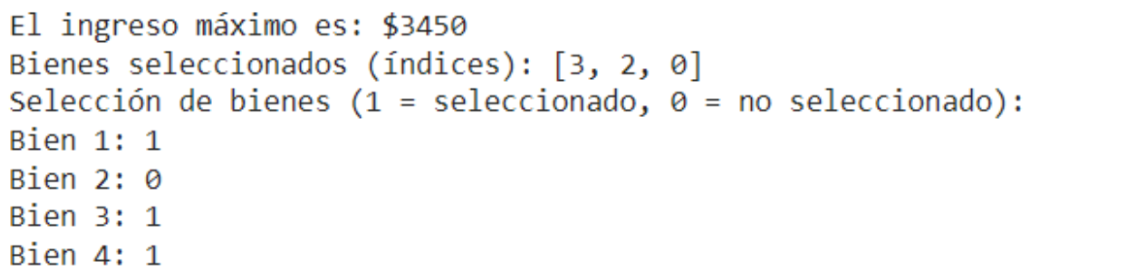
\includegraphics[width=0.8\textwidth]{resultado_mochila_ejem2.png}
    \caption{Imagen del resultado del código Python.}
    \label{fig:resultado_ejemplo2}
\end{figure}

\subsubsection{Análisis de complejidad}
\begin{figure}[H]
    \centering
    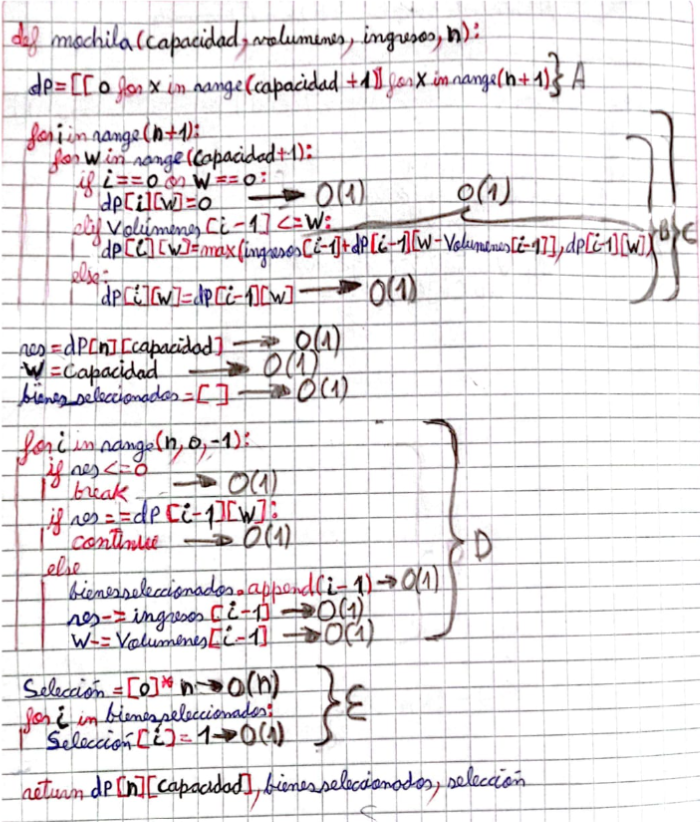
\includegraphics[width=0.8\textwidth]{complejidad_mochila_ejem2.png}
    \caption{Análisis del código.}
    \label{fig:complejidad_ejemplo2}
\end{figure}

\begin{figure}[H]
    \centering
    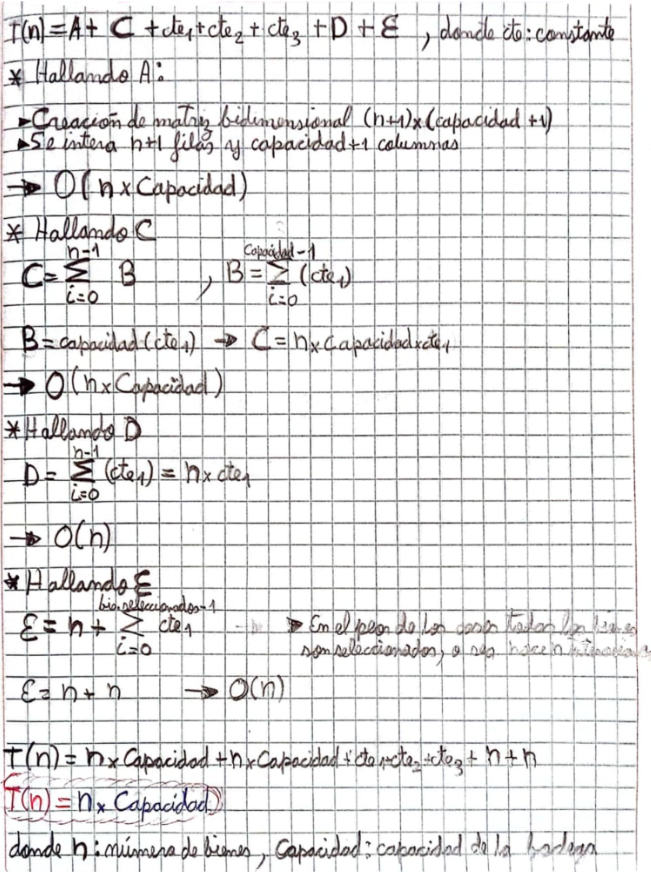
\includegraphics[width=0.8\textwidth]{complejidad_mochila_ejem2_2.png}
    \caption{Análisis del código.}
    \label{fig:complejidad_ejemplo2_2}
\end{figure}

Como se acaba de apreciar, el presente algoritmo tiene una complejidad aproximada de O(n x K) o, equivalentemente, n x capacidad, lo cual supone eficiencia en función al dato de entrada de “capacidad”; mientras más sea esto, más complejo se vuelve.

\section{El Problema de las Distancias Más Cortas}
El problema de las distancias más cortas es uno de los temas más estudiados en la teoría de grafos por sus numerosas aplicaciones, incluyendo la ingeniería de redes, la logística, inteligencia artificial y la investigación operativa. El problema trata sobre un grafo que es una estructura compuesta por nodos y aristas. Cada arista es una conexión entre vértices y puede tener un peso asociado que representa la "distancia" o el "costo" de viajar entre dichos nodos. Se desea hallar la ruta de menor coste entre dos nodos.

\subsection{Ejemplo 1}
\textbf{Algoritmo de Floyd Warshall}
Imaginemos la situación de un repartidor de agua que decide crear una red de entrega de suministros a domicilio con la intención de repartir sus pedidos en el menor tiempo posible. Inicialmente sólo opera únicamente en seis casas, que puedes cubrir gracias a la facilidad de desplazarse entre ellas.
Sin embargo, desea encontrar las rutas más cortas a seguir entre su local y la de sus clientes para cumplir con las entregas de la manera más óptima. Por ello, realizamos el análisis para saber todas las posibles rutas que utilizaría el repartidor.
%%%%%%%%%
\begin{figure}[H]
	\centering
	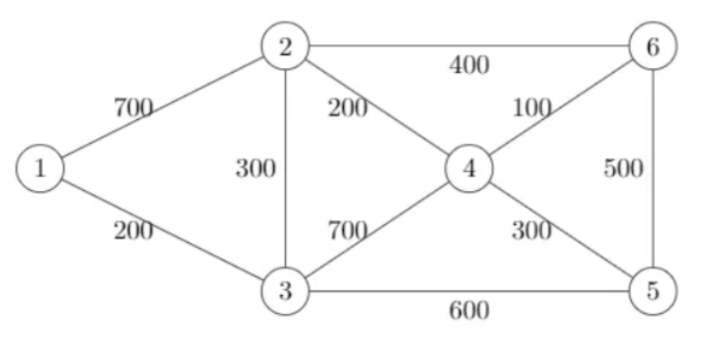
\includegraphics[width=0.8\textwidth]{distancias_cortas_RepresentacionG1.png}
	\caption{Representación gráfica del problema.}
	\label{fig:resultado1}
\end{figure}

Uno de los algoritmos más utilizados en programación dinámica para este tipo de problemas es el algoritmo de Floyd Warshall, cuyo pseudocódigo es el siguiente
%%%%%%%%%
\begin{figure}[H]
	\centering
	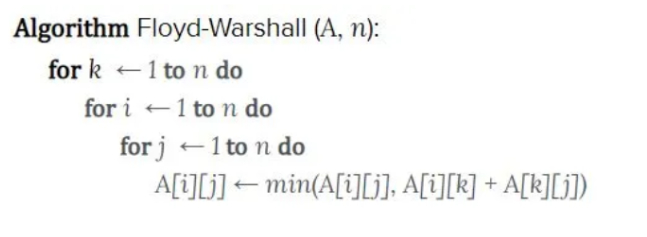
\includegraphics[width=0.8\textwidth]{distancias_cortas_Pseudo1.png}
	\caption{Pseudocódigo de Floyd Warshall.}
	\label{fig:resultado2}
\end{figure}

\subsubsection{Código}
\begin{lstlisting}
	import sys
	INF = sys.maxsize
	#Implementacion
	def Floyd_Warshall(graph):
	n = len(graph)
	dist = [[] for i in range(n)]
	for i in range(n):
	for j in range(n):
	dist[i].append(graph[i][j]) #inicializar matriz de distancias
	
	for k in range(n):
	for i in range(n):
	for j in range(n):
	dist[i][j] = min(dist[i][j], dist[i][k] + dist[k][j])
	#Imprimir solucion
	print('Distancia mas corta entre todo par de nodos:')
	for i in range(n):
	for j in range(n):
	if dist[i][j] == INF:
	print("%7s" % ("INF"), end = ' ')
	else:
	print("%7s" % (dist[i][j]), end = ' ')
	print()
	#Grafo
	graph = [ [0, 700, 200, INF, INF, INF],
	[700, 0, 300, 200, INF, 400],
	[200, 300, 0, 700, 600, INF],
	[INF, 200, 700, 0, 300, 100],
	[INF, INF, 600, 300, 0, 500],
	[INF, 400, INF, 100, 500, 0]
	]
	Floyd_Warshall(graph)
	
\end{lstlisting}

\subsubsection{Resultado}
%%%%%%%%%
\begin{figure}[H]
	\centering
	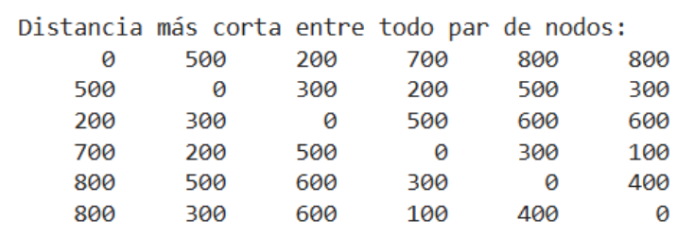
\includegraphics[width=0.8\textwidth]{resultado_distancias_ejem1.png}
	\caption{Resultado de la ejecución del código Python.}
	\label{fig:resultado3}
\end{figure}

\subsubsection{Análisis de complejidad}

\section*{Análisis de Complejidad}

\subsection*{Detalle de Complejidad}

El código correspondiente es:
\begin{lstlisting}
	def Floyd_Warshall(graph):
	n = len(graph) #... O(1)
	dist = [[] for i in range(n)] #... O(n)
	for i in range(n): #...Q
	  for j in range(n): #...P
		dist[i].append(graph[i][j]) #...O(1)
  
	for k in range(n): #...T
	  for i in range(n): #...S
		for j in range(n): #...R
		  dist[i][j] = min(dist[i][j], dist[i][k] + dist[k][j]) #...O(1)
	#Imprimir solucion
	print('Distancia mas corta entre todo par de nodos:') #...O(1)
	for i in range(n): #...V
	  for j in range(n): #...U
		if dist[i][j] == INF: #...O(1)
		  print("%7s" % ("INF"), end = ' ') #...O(1)
		else:
		  print("%7s" % (dist[i][j]), end = ' ') #...O(1)
	  print() #...O(1)

\end{lstlisting}

\subsection*{Complejidad Total}
\subsection*{Fórmula }
La complejidad del codigo se determina de la siguiente manera
\[T(n) = 1 + n + n + Q + T + 1 + V\]
\[ Q = \sum_{i = 1}^{\\n} P \quad T = \sum_{k = 1}^{\\n} S \quad V = \sum_{i = 1}^{\\n} U \]

Entonces
\[T(n) = 1 + n + n + \sum_{i = 1}^{\\n} P + \sum_{k = 1}^{\\n} S  + 1 + \sum_{i = 1}^{\\n} U \]
\[P = \sum_{j = 1}^{\\n} 1 \quad S = \sum_{i = 1}^{\\n} R\ \quad U = \sum_{j = 1}^{\\n} (1+1+1) \]
\[T(n) = 2 + 2n + \sum_{i = 1}^{\\n} \sum_{j = 1}^{\\n} 1 + \sum_{k = 1}^{\\n} \sum_{i = 1}^{\\n} R + \sum_{i = 1}^{\\n} \sum_{j = 1}^{\\n} (1 + 1 + 1) \]
\[T(n) = 2 + 2n + n^2 + \sum_{k = 1}^{\\n} \sum_{i = 1}^{\\n} \sum_{j = 1}^{\\n} 1 + 3n^2 \]
\[T(n) = 2 + 2n + n^2 + n^3 + 3n^2 \]
\[T(n) = 2 + 2n + 4n^2 + n^3 \]
\[T(n) = O(n^3)\]

Como es posible apreciar, el uso del algoritmo tiene un costo aproximado de O($n^3$), lo cual no representa muy favorable en términos de eficiencia.

\subsection*{Variables}

\begin{itemize}
    \item \( n \) = número de vertices.
\end{itemize}

\subsection{Ejemplo 2}
\textbf{Algoritmo de Bellman-Ford}

Eres ingeniero de sistemas especializado en redes en una empresa en la que trabajas. Se calculan los tiempos que demoran para comunicarse entre distintos routers. Se te pide por tanto hallar el menor tiempo posible para comunicarte desde el Router Riobamba hacia todos los demás routers. 

%%%%%%%%%
\begin{figure}[H]
	\centering
	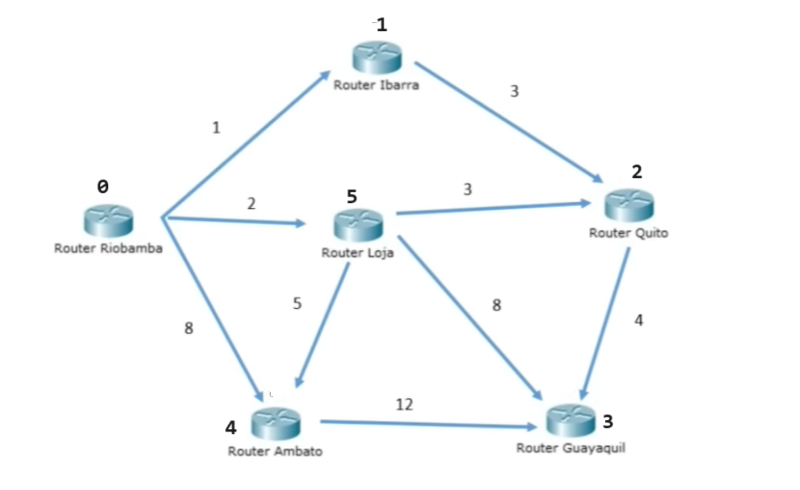
\includegraphics[width=0.8\textwidth]{bellman-fordejemplo.png}
	\caption{Representación gráfica del problema.}
	\label{fig:resultado4}
\end{figure}


Uno de los algoritmos más utilizados en programación dinámica para este tipo de problemas es el algoritmo de Bellman-Ford, cuyo pseudocódigo es el siguiente:

%%%%%%%%%
\begin{figure}[H]
	\centering
	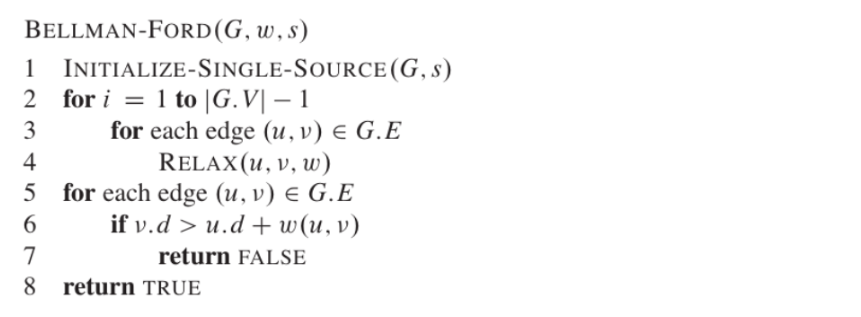
\includegraphics[width=0.8\textwidth]{distancias_cortas_Pseudo2.png}
	\caption{Pseudocódigo de Bellman-Ford.}
	\label{fig:resultado5}
\end{figure}

\subsubsection{Código}
\begin{lstlisting}[language=Python]
	#Diccionario de aristas y sus pesos
	w = {
		(0,1) : 1,
		(0,5) : 2,
		(0,4) : 8,
		(1,2) : 3,
		(2,3) : 4,
		(4,3) : 12,
		(5,2) : 3,
		(5,3) : 8,
		(5,4) : 5
	}
	
	#numero de vertices
	n = 6
	
	def relax (u,v,w,d,p):
	if d[v] > d[u] + w[u,v]:
	d[v] = d[u] + w[u,v]
	p[v] = u
	
	def Bellman_Ford(w,n,s):
	
	inf = 1e100
	d = [0 for i in range(n)] ##Es la cota superior del peso del camino mas corto de s a v, se inicializa en infinito
	p = [0 for i in range(n)] ##Es el nodo previo en el camino del peso mas corto de s a v
	
	for vertex in range(n):
	d[vertex] = inf #Asumimos infinito al principio, es decir, es desconocido el limite
	p[vertex] = 'null' #Aun no sabemos el nodo previo de vertex en el camino mas corto
	
	d[s] = 0 #0 porque el peso de s a s es 0
	
	for _ in range (n-1):
	for u,v in w:  #arista (u,v) : peso
	relax(u,v,w,d,p) #actualizacion de las distancias
	
	for (u,v) in w: #detectar ciclos negativos
	if d[v] > d[u] + w[u,v]:
	return False
	
	print("Distancias mas cortas")
	for i in range(n):
	print(i, ": ", d[i])
	
	print("\nNodos previos")
	for i in range(n):
	print(i, ": ", p[i])
	
	return True
	
	Bellman_Ford(w,n,0)
	
\end{lstlisting}

\subsubsection{Resultado}
%%%%%%%%%%
\begin{figure}[H]
	\centering
	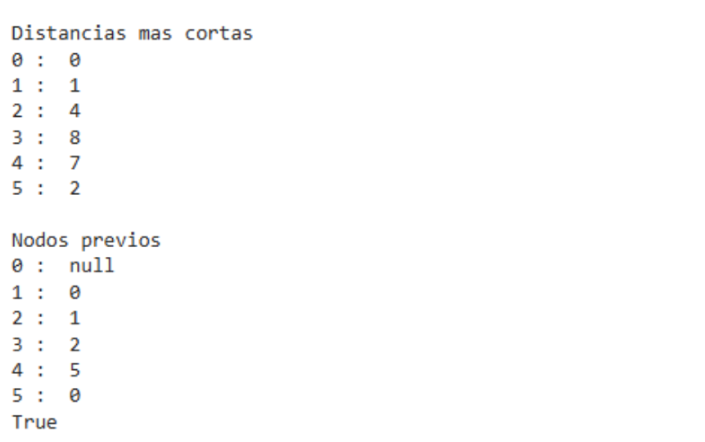
\includegraphics[width=0.8\textwidth]{resultado_distancias_ejem2.png}
	\caption{Resultado de la ejecución del codigo Python.}
	\label{fig:resultado6}
\end{figure}

\subsubsection{Análisis de complejidad}

\section*{Análisis de Complejidad}

\subsection*{Detalle de Complejidad}

El código correspondiente es:
\begin{lstlisting}
	def relax (u,v,w,d,p): #...A
	if d[v] > d[u] + w[u,v]: #...O(1)
	  d[v] = d[u] + w[u,v]	#...O(1)
	  p[v] = u	#...O(1)
  
  def Bellman_Ford(w,n,s):
  
	inf = 1e100 #...O(1)
	d = [0 for i in range(n)] #...O(n)
	p = [0 for i in range(n)] #...O(n)
  
	for vertex in range(n): #...P
	  d[vertex] = inf #...O(1)
	  p[vertex] = 'null' #...O(1)
  
	d[s] = 0 #...O(1)
  
	for _ in range (n-1): #...Q
	  for u,v in w:  #...R
		relax(u,v,w,d,p) #...A
  
	for (u,v) in w:  #...S
	  if d[v] > d[u] + w[u,v]: #...O(1)
		return False #...O(1)
  
	print("Distancias mas cortas") #...O(1)
	for i in range(n): #...O(n)
	  print(i, ": ", d[i])
  
	print("\nNodos previos") #...O(1)
	for i in range(n): #...O(n)
	  print(i, ": ", p[i])
  
	return True #...O(1)

\end{lstlisting}

\subsection*{Complejidad Total}
\subsection*{Fórmula }
La complejidad del codigo se determina de la siguiente manera
\[relax \Longrightarrow A = O(1)\]
\[T(n) = 1 + n + n + P + 1 + Q + S + 1 + n + 1 + n + 1 \]
\[T(n) = 5 + 4n + P + Q + S \]
\[P = \sum_{i = 1}^{\\n} 2 \quad Q = \sum_{i = 1}^{\\n-1} R \quad S = \sum_{aristas \epsilon W }^{} 1 \]
\[T(n) = 5 + 4n + \sum_{i = 1}^{\\n} 2 + \sum_{i = 1}^{\\n-1} R + \sum_{aristas \epsilon W }^{} 1 \]
\[R = \sum_{aristas \epsilon W }^{} A \]
\[T(n) = 5 + 4n + (2n) + \sum_{i = 1}^{\\n-1} \sum_{aristas \epsilon W }^{} A + m\]
\[T(n) = 5 + 6n + \sum_{i = 1}^{\\n-1} \sum_{aristas \epsilon W }^{} 1 + m\]
\[T(n) = 5 + 6n + \sum_{i = 1}^{\\n-1} m + m\]
\[T(n) = 5 + 6n + m(n-1) + m\]
\[T(n) = mn + 6n + 5\]
\[T(n) = O(m*n)\]

El uso del algoritmo tiene un costo aproximado de O(m*n). Si m fuese el numero maximo de aristas la complejidad pasaria a ser de O($n^3$)

\subsection*{Variables}

\begin{itemize}
    \item \( n \) = número de vertices.
    \item \( m \) = número de aristas.
\end{itemize}


\section{Conclusiones}
La programación dinámica se demuestra como una herramienta poderosa y versátil para resolver problemas de optimización clásicos como el cambio de monedas, el problema de la mochila y el problema de las distancias más cortas. A través de los ejemplos y análisis realizados, se evidencia su aplicabilidad en diferentes contextos, así como la importancia de entender la complejidad algorítmica para mejorar la eficiencia de las soluciones propuestas.

\input{referencias}

\end{document}
